\section*{\Large{Введение}}
В современном мире каждая компания хочет минимизировать свои
затраты, как по времени, так и в финансовом плане.
Это не обошло и сферу строительства.
В данной области существует ряд открытых задач, требующих решения,
в том числе это касается сферы проектирования генеральных планов площадных объектов.


Любоe сооружение несет в себе определенную функцию. Склады служат для хранения вещей, факелы для сжигания
попутного газа, а нефтеперерабатывающий завод для преобразования сырой нефти в нефтепродукты.
Чем сложнее задача, которую решает промышленный объект,
тем сложнее он устроен, и из большего числа сооружений он состоит.
А чем больше сооружений находится рядом, тем больше появляется различных ограничений,
продиктованных вопросами безопасности строительства этих зданий рядом друг с другом.


Крайне опасно размещать факел для сжигания попутного рядом с хранилищем топлива из-за высокой пожароопасности хранилища.
В случае возгорания хранилища, топливо, которое находится в нём, может быть не только огнеоопасным, но также
и взрывоопасным. Соответственно, если в зоне поражения взрыва находятся сооружения, требующие постоянного присутствия людей,
то помимо повреждения материальных объектов, могут погибнуть или быть травмированы люди, чего допускать никак нельзя.



Для того, чтобы минимизировать риски возникновения нештатных ситуаций, повреждения материального имущества, а также, что
является самым важным, риск возникновения несчастных случаев


\par
\begin{figure}[H]
	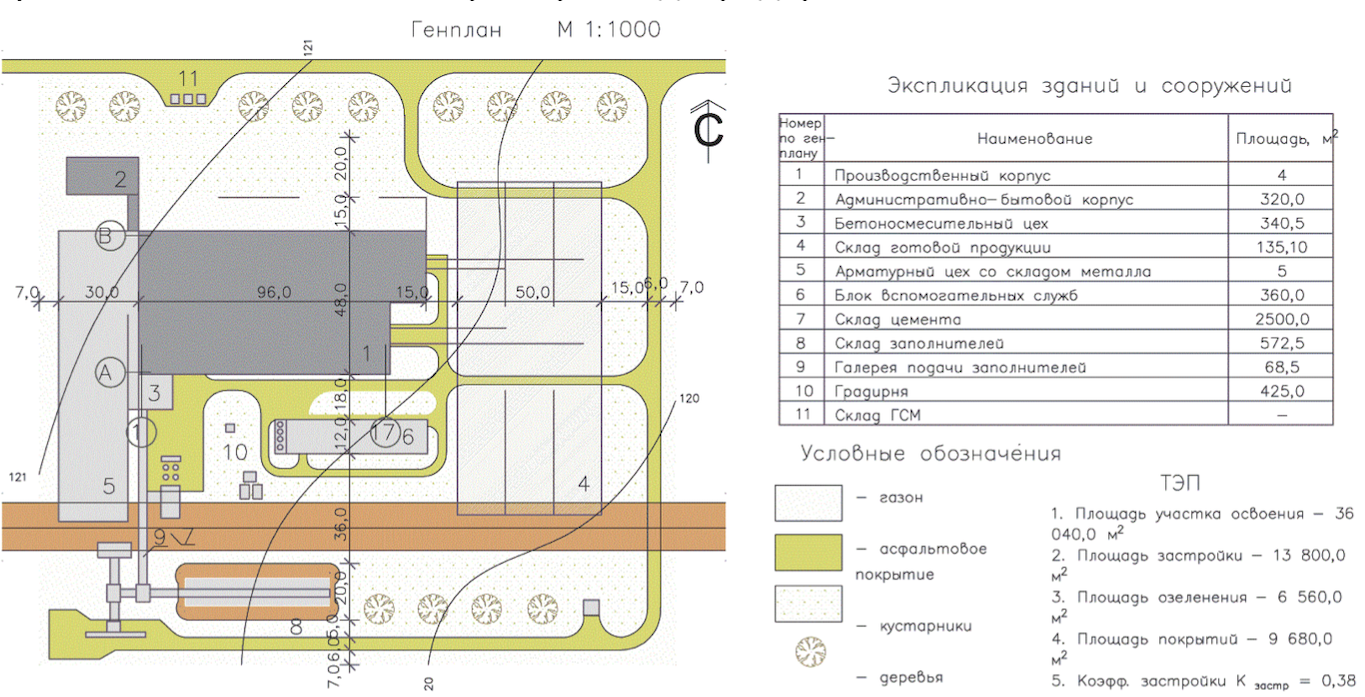
\includegraphics[width=0.9\textwidth]{images/introduction/1}
	\caption{Генеральный план завода}
	\label{pic:introduction__site_plan}
\end{figure}
\par

